\chapter{Технологический раздел}
\label{cha:impl}

Далее в технологическом разделе будут описаны выбранные технологии разработки, методология построения ПО, а также рассмотрено взаимодействие пользователя с приложением.


\section{Выбор технологий разработки}

В качестве СУБД был сделан выбор в пользу PostgreSQL --- это мощная система объектно-реляционных баз данных с открытым исходным кодом, которая использует и расширяет язык SQL в сочетании со многими функциями, позволяющими безопасно хранить и масштабировать самые сложные рабочие нагрузки данных \cite{postgre}.

В качестве ЯП был сделан выбор в пользу Go --- это проект с открытым исходным кодом, призванный повысить продуктивность программистов. Язык Go выразительный, лаконичный, чистый и эффективный. Его механизмы параллелизма упрощают написание программ, максимально использующих многоядерные и сетевые машины, а новая система типов обеспечивает гибкое и модульное построение программ. Go быстро компилируется в машинный код, но обладает удобством сборки мусора и возможностями отражения во время выполнения. Это быстрый, статически типизированный компилируемый язык, который выглядит как динамически типизированный интерпретируемый язык \cite{golang}.

Для разработки программного интерфейса используется Fyne --- это простая в освоении бесплатная платформа с открытым исходным кодом для создания графических приложений для настольных компьютеров, мобильных устройств и других устройств. Сочетая мощь и простоту языка программирования Go с тщательно продуманной библиотекой виджетов разработчику легко создавать приложения и развертывать их \cite{fyne}.

\section{Методология построения ПО}

Разрабатываемое приложение спроектировано на основе чистой архитектуры. Этот способ организации кода подразумевает четкое строгое разделение ответственности. Приложение разбивается на независимые функциональные компоненты, которые взаимодействуют друг с другом определенным образом, при этом между ними передаются только те ресурсы, которые необходимы для выполнения конкретной задачи. Это помогает минимизировать сложность каждого компонента, снизить вероятность ошибок и ускоряет их выявление \cite{cleancode}.

На рисунке \ref{fig:components} представлено высокоуровневое разбиение приложения на компоненты. Данный подход позволяет легко масштабировать приложение, а также выполнять подмену независимых компонентов, не привязываясь к их конкретной реализации.

\begin{figure}[h!btp]
	\centering
	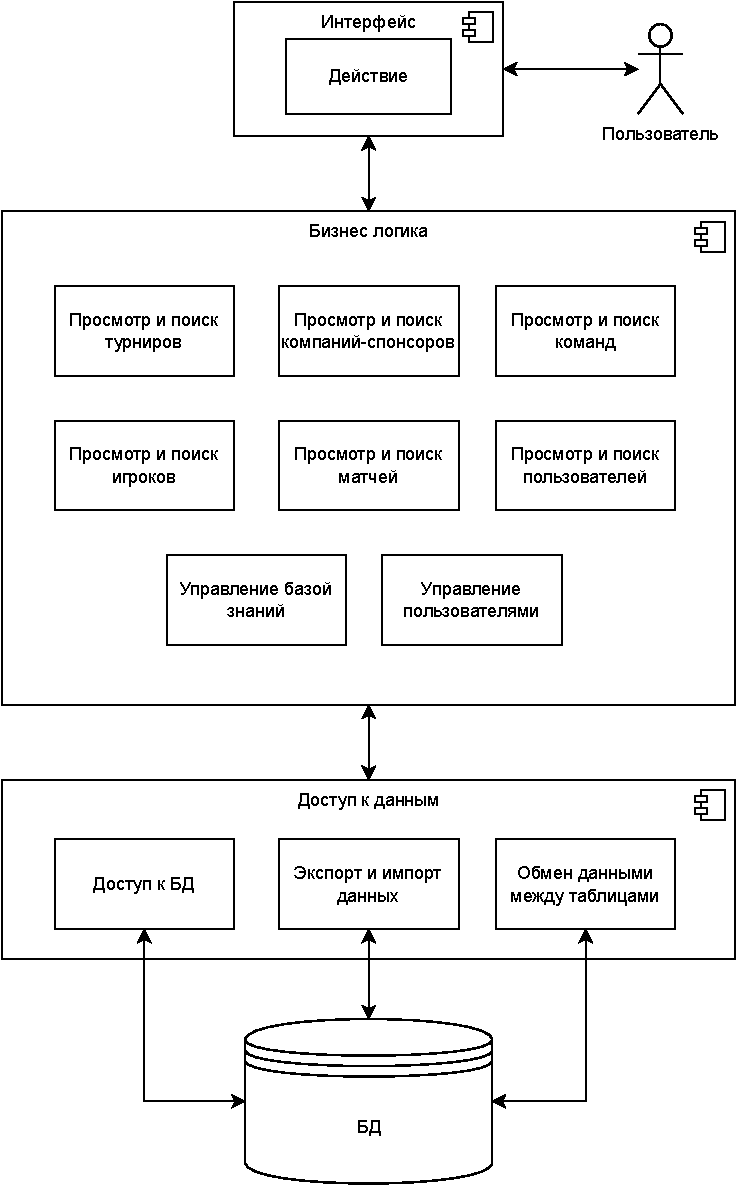
\includegraphics[scale = 0.9]{inc/diag/components.pdf}
	\caption{Высокоуровневое разбиение на компоненты}
	\label{fig:components}	
\end{figure}

\clearpage


\section{Описание интерфейса программного продукта}


При запуске приложения пользователю предоставляется возможность регистрации и создания собственного аккаунта в системе или выполнить вход под уже имеющимся (рисунок \ref{fig:login}).

\begin{figure}[h!btp]
	\centering
	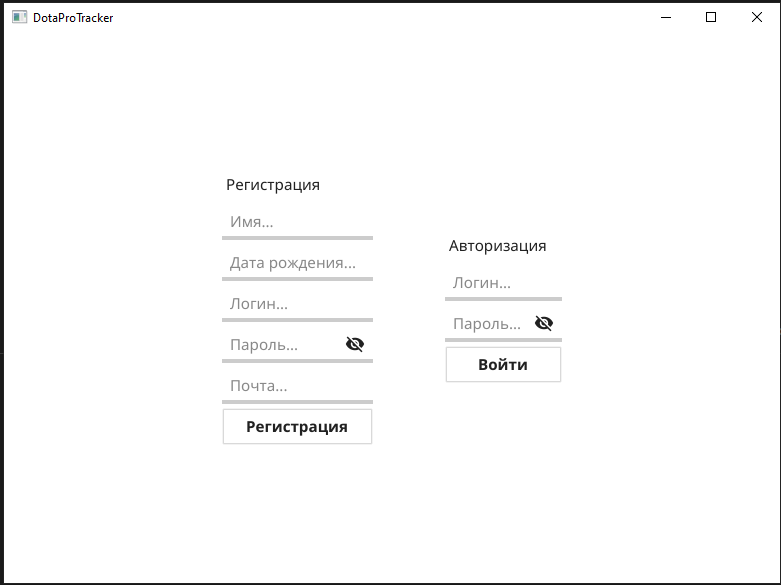
\includegraphics[scale = 0.7]{inc/img/login.png}
	\caption{Стартовое окно приложения}
	\label{fig:login}	
\end{figure}

После выполнения процедуры идентификации происходит процедура аутентификации пользователя (выполняется проверка соотвествия пароля введенного пользователем, с соответствующим паролем в базе данных, следует отметить, что пароли хранятся в зашифрованном виде с целью обеспечения сохранности и безопасности данных пользователей). В случае успешной аутентификации, пользователь получает доступ к функциям системы на основе своего уровня привилегий. На рисунке \ref{fig:admin} изображен интерфейс администратора.

\clearpage

\begin{figure}[h!btp]
	\centering
	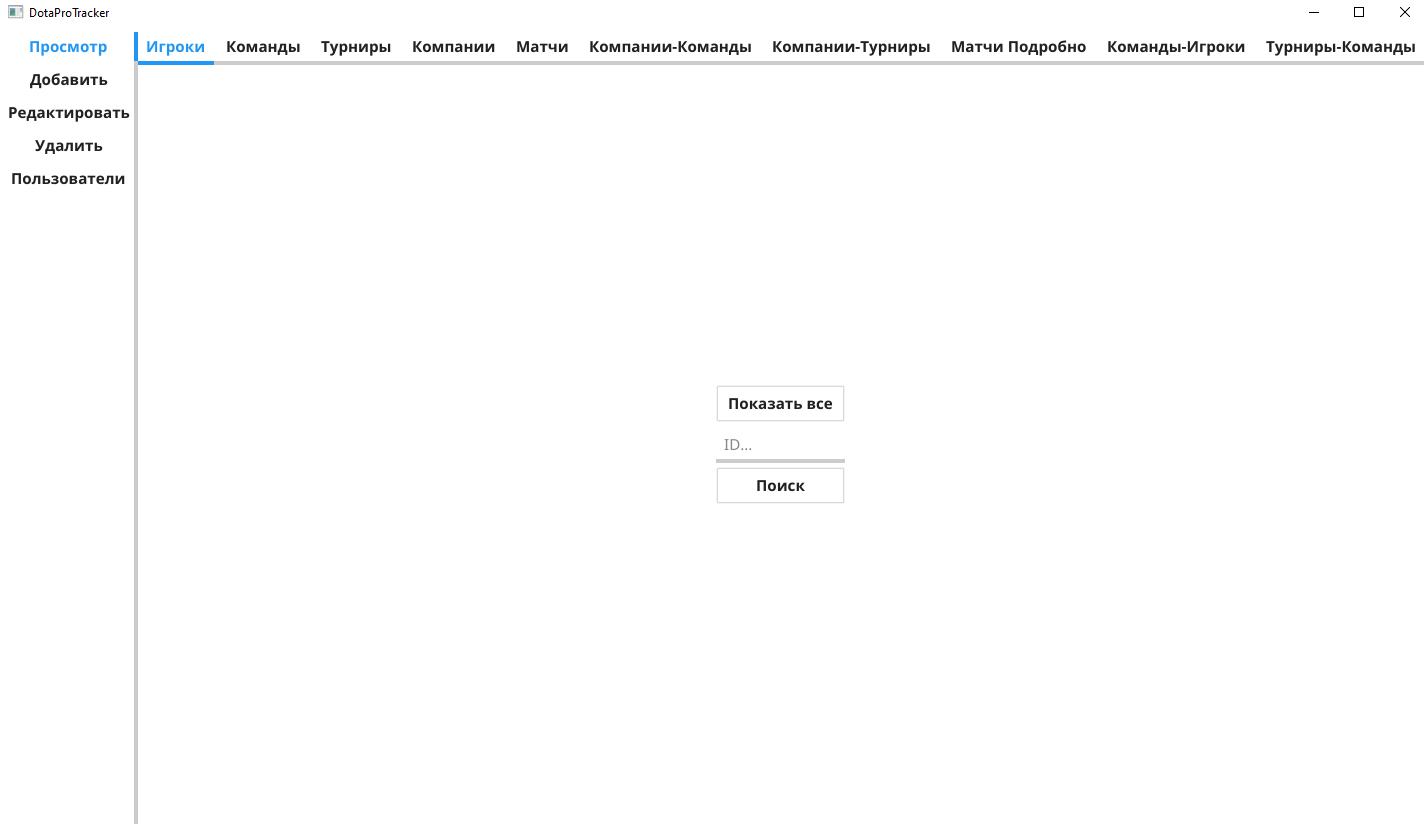
\includegraphics[scale = 0.4]{inc/img/admin.png}
	\caption{Интерфейс администратора}
	\label{fig:admin}	
\end{figure}

Администратор системы имеет право добавлять новых пользователей в систему, а также смотреть весь список существующих аккаунтов (рисунки \ref{fig:user_create}--\ref{fig:users}).


\begin{figure}[h!btp]
	\centering
	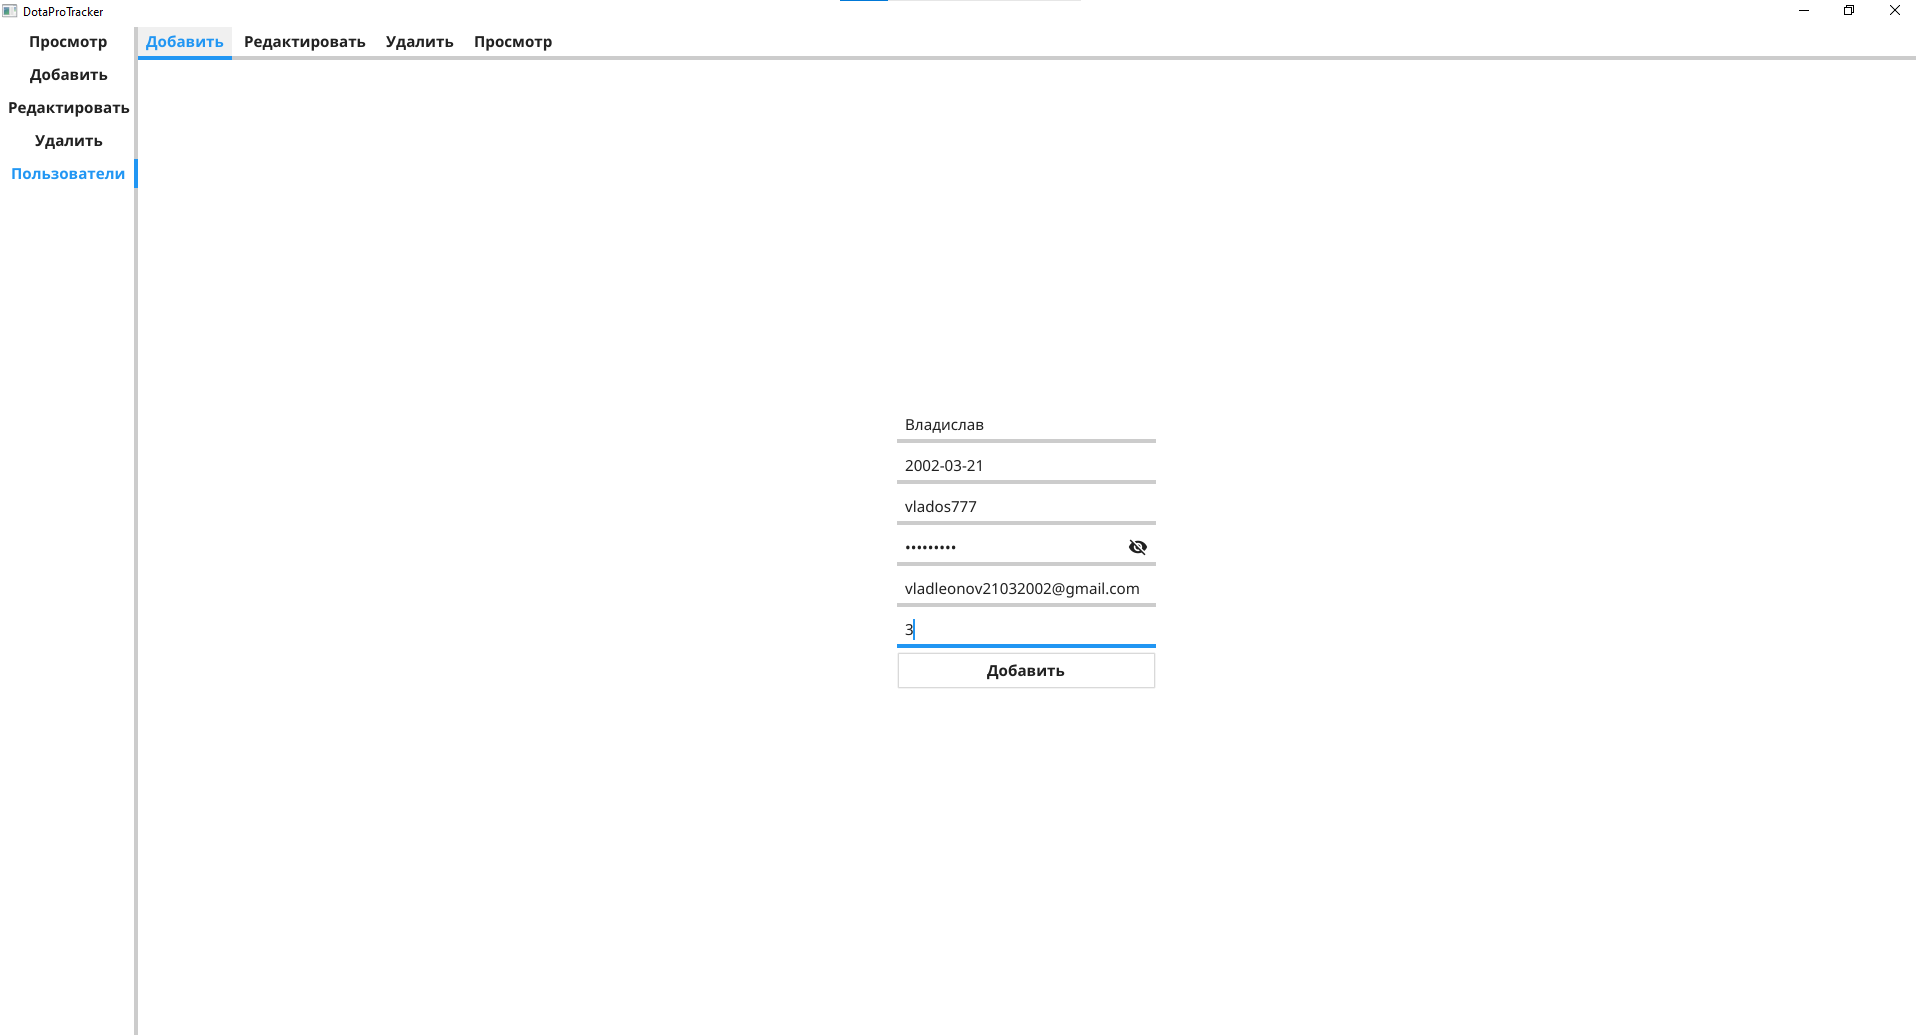
\includegraphics[scale = 0.3]{inc/img/user_create.png}
	\caption{Создание нового пользователя}
	\label{fig:user_create}	
\end{figure}


\clearpage

\begin{figure}[h!btp]
	\centering
	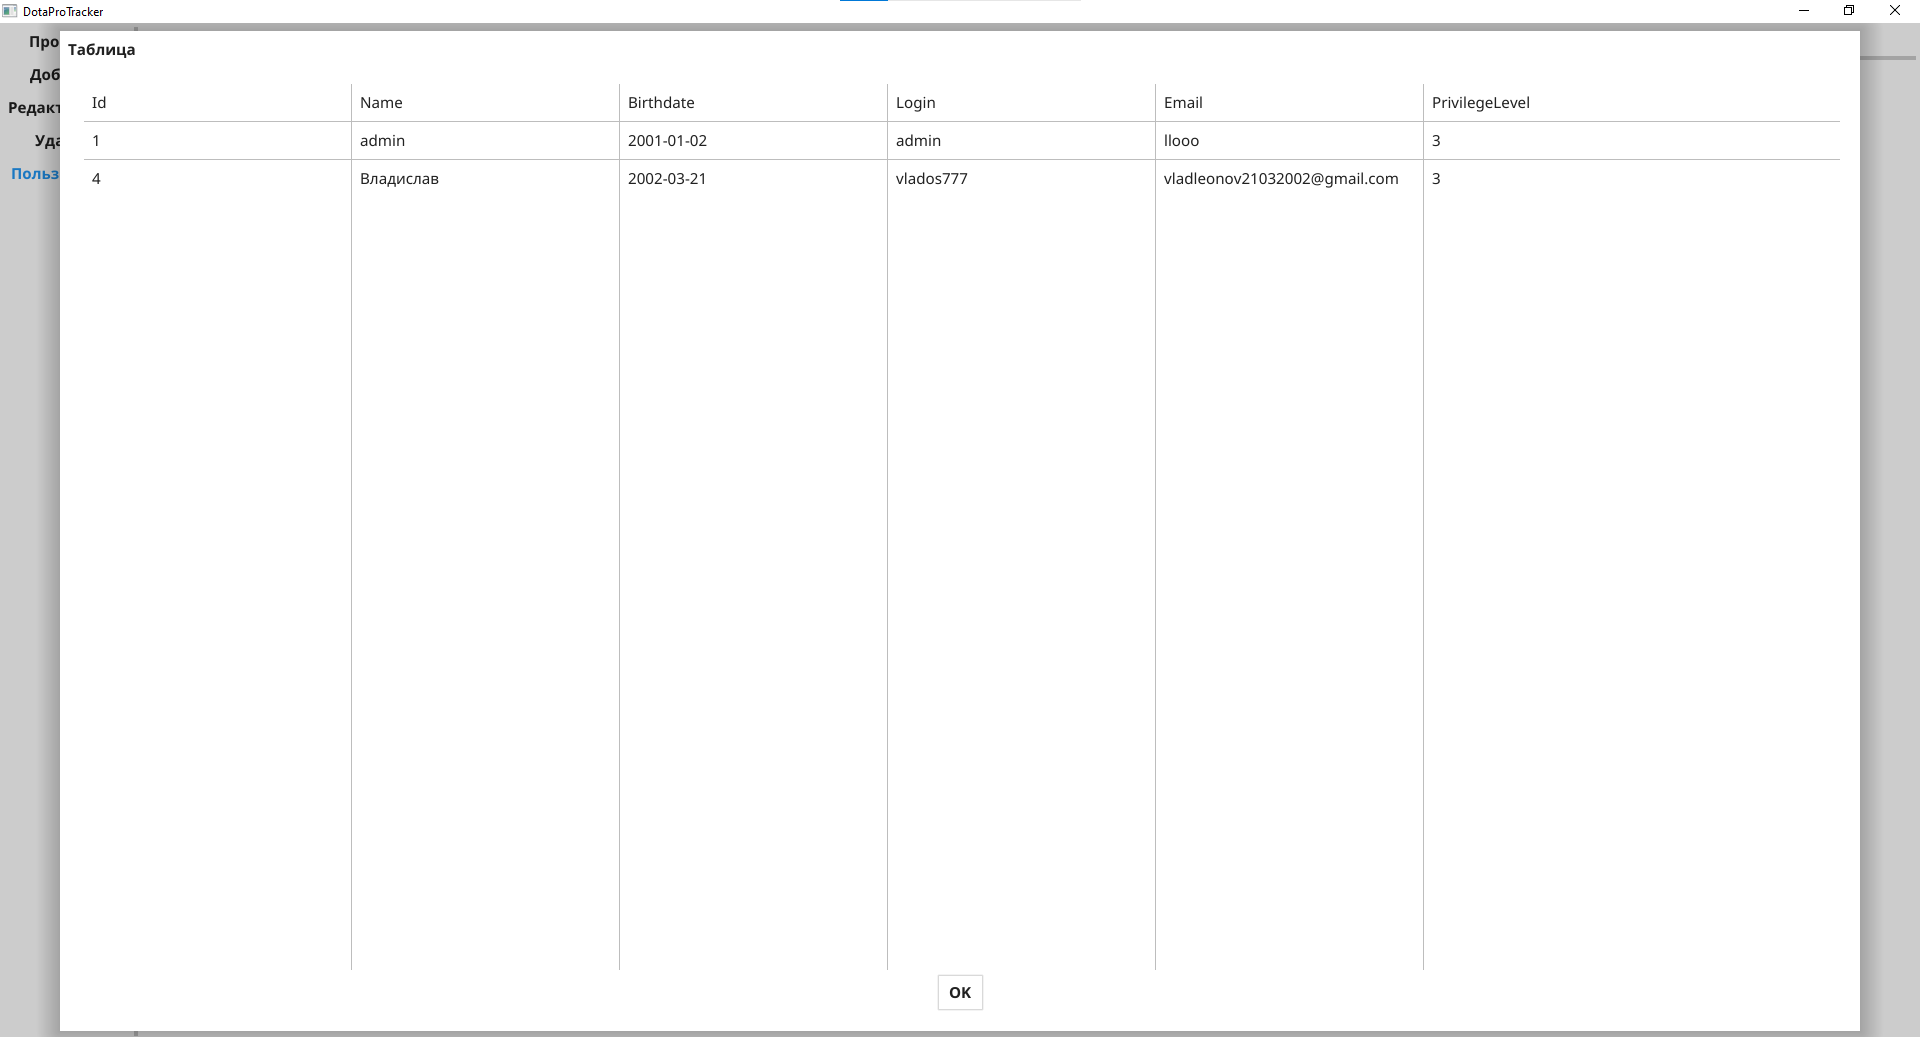
\includegraphics[scale = 0.3]{inc/img/users.png}
	\caption{Список существующих пользователей}
	\label{fig:users}	
\end{figure}

Роль модератора позволяет редактировать записи системы. Для навигации по записям реализована функция поиска (рисунки \ref{fig:edit}--\ref{fig:find})

\begin{figure}[h!btp]
	\centering
	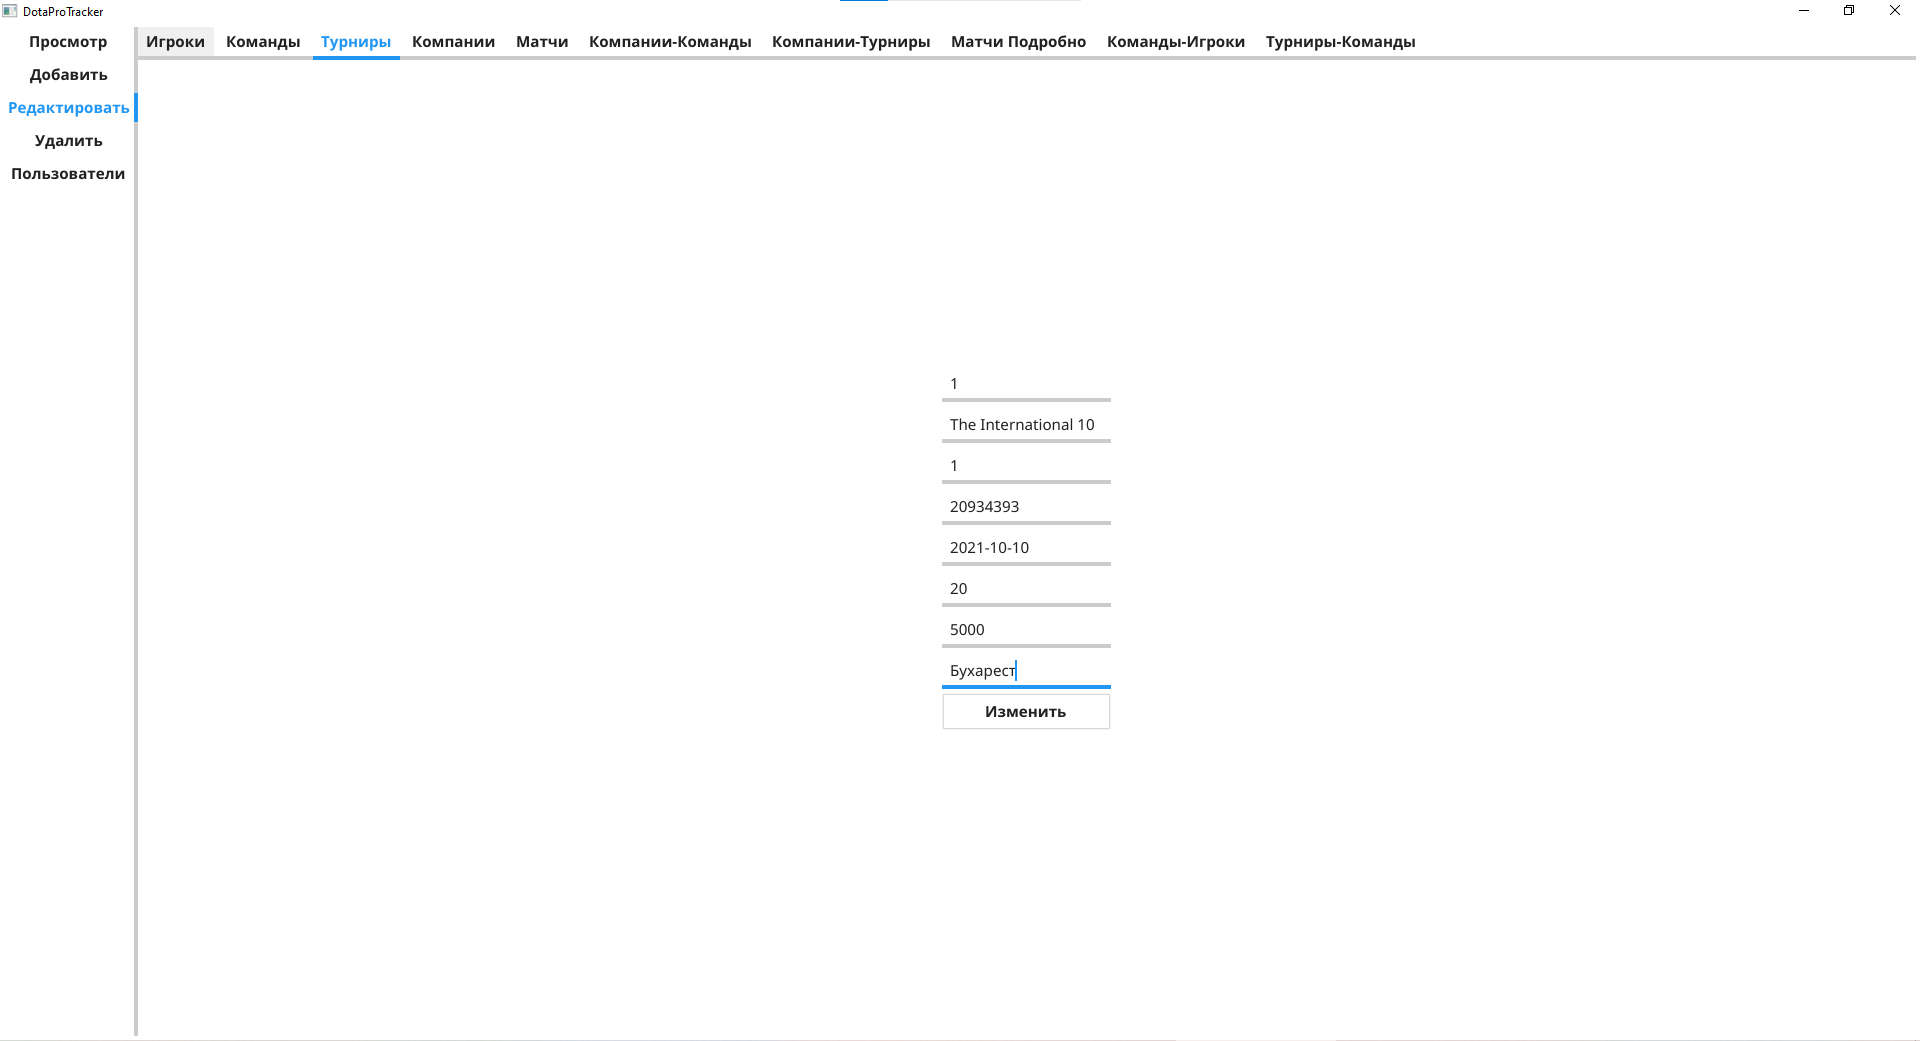
\includegraphics[scale = 0.3]{inc/img/edit.png}
	\caption{Редактирование записи о турнире}
	\label{fig:edit}	
\end{figure}

\clearpage

\begin{figure}[h!btp]
	\centering
	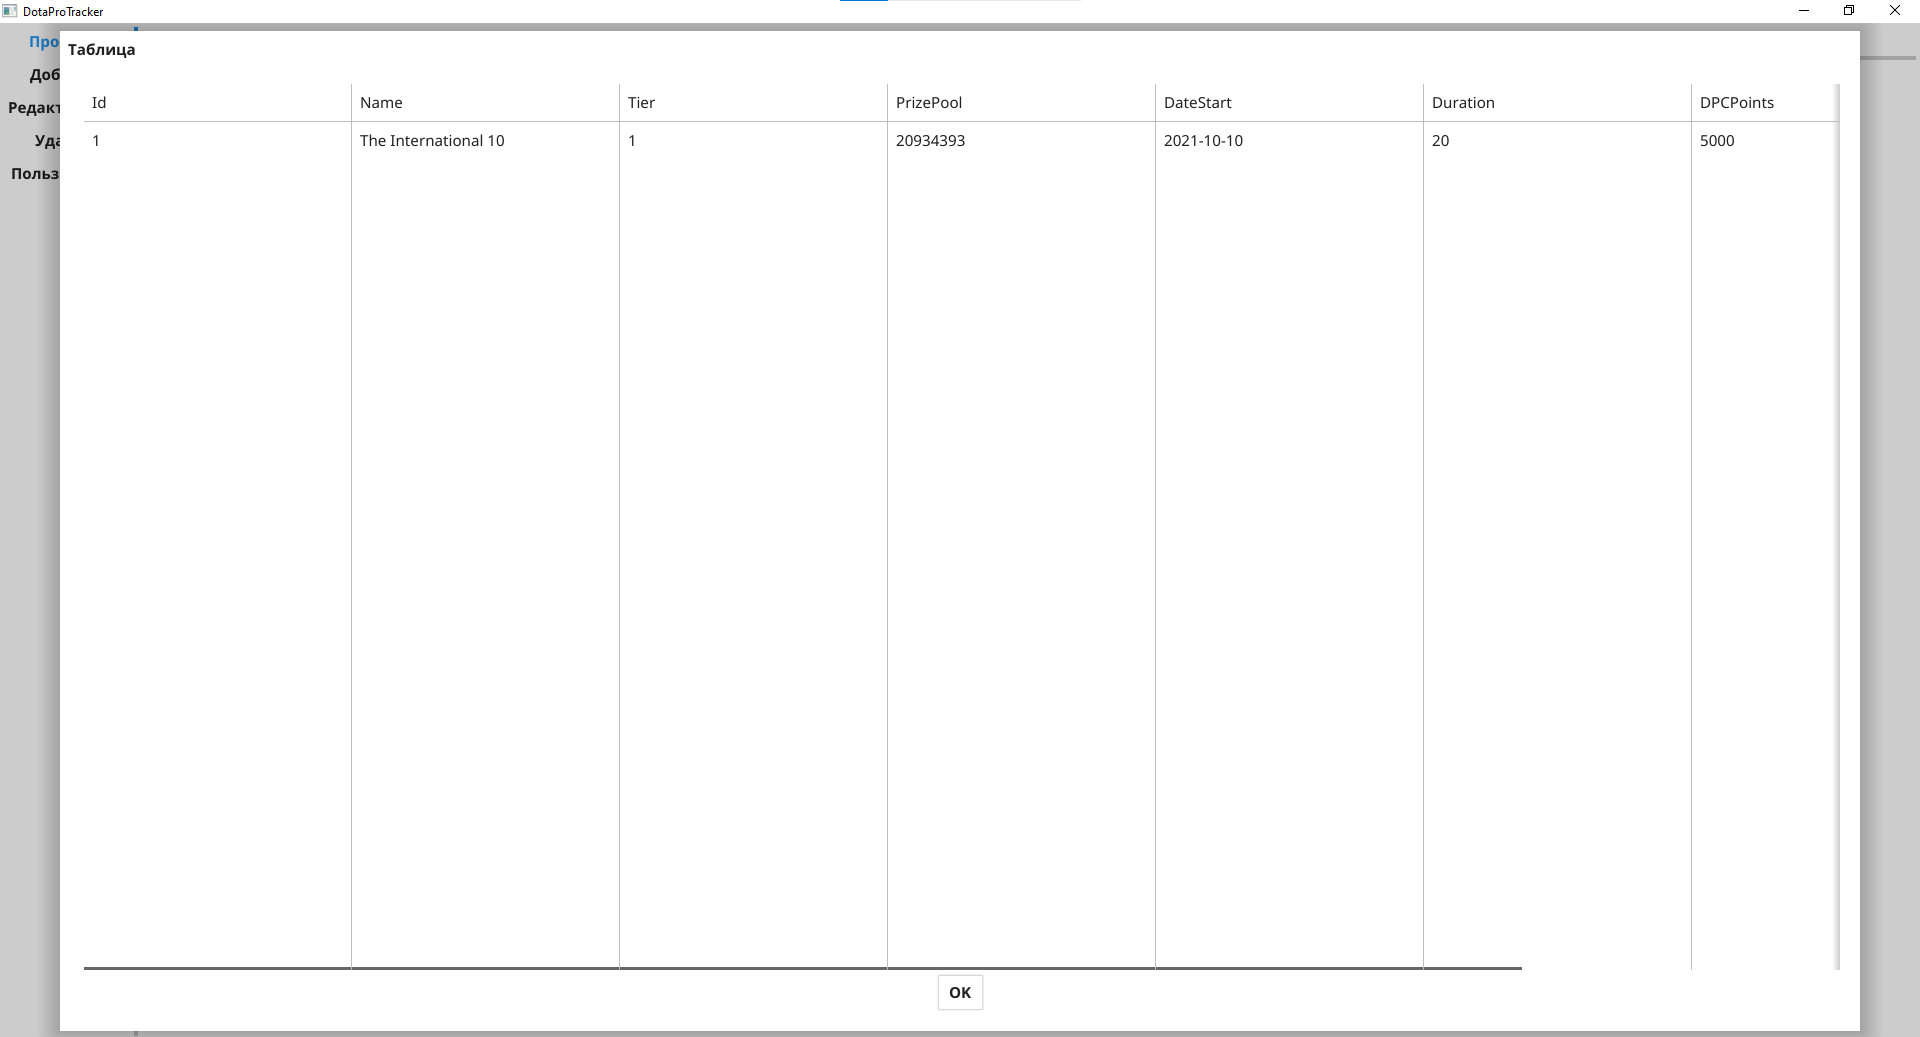
\includegraphics[scale = 0.3]{inc/img/find.png}
	\caption{Поиск записи о турнире}
	\label{fig:find}	
\end{figure}

Обычный пользователь имеет возможность просмотра и поиска записей (рисунок \ref{fig:companies}).

\begin{figure}[h!btp]
	\centering
	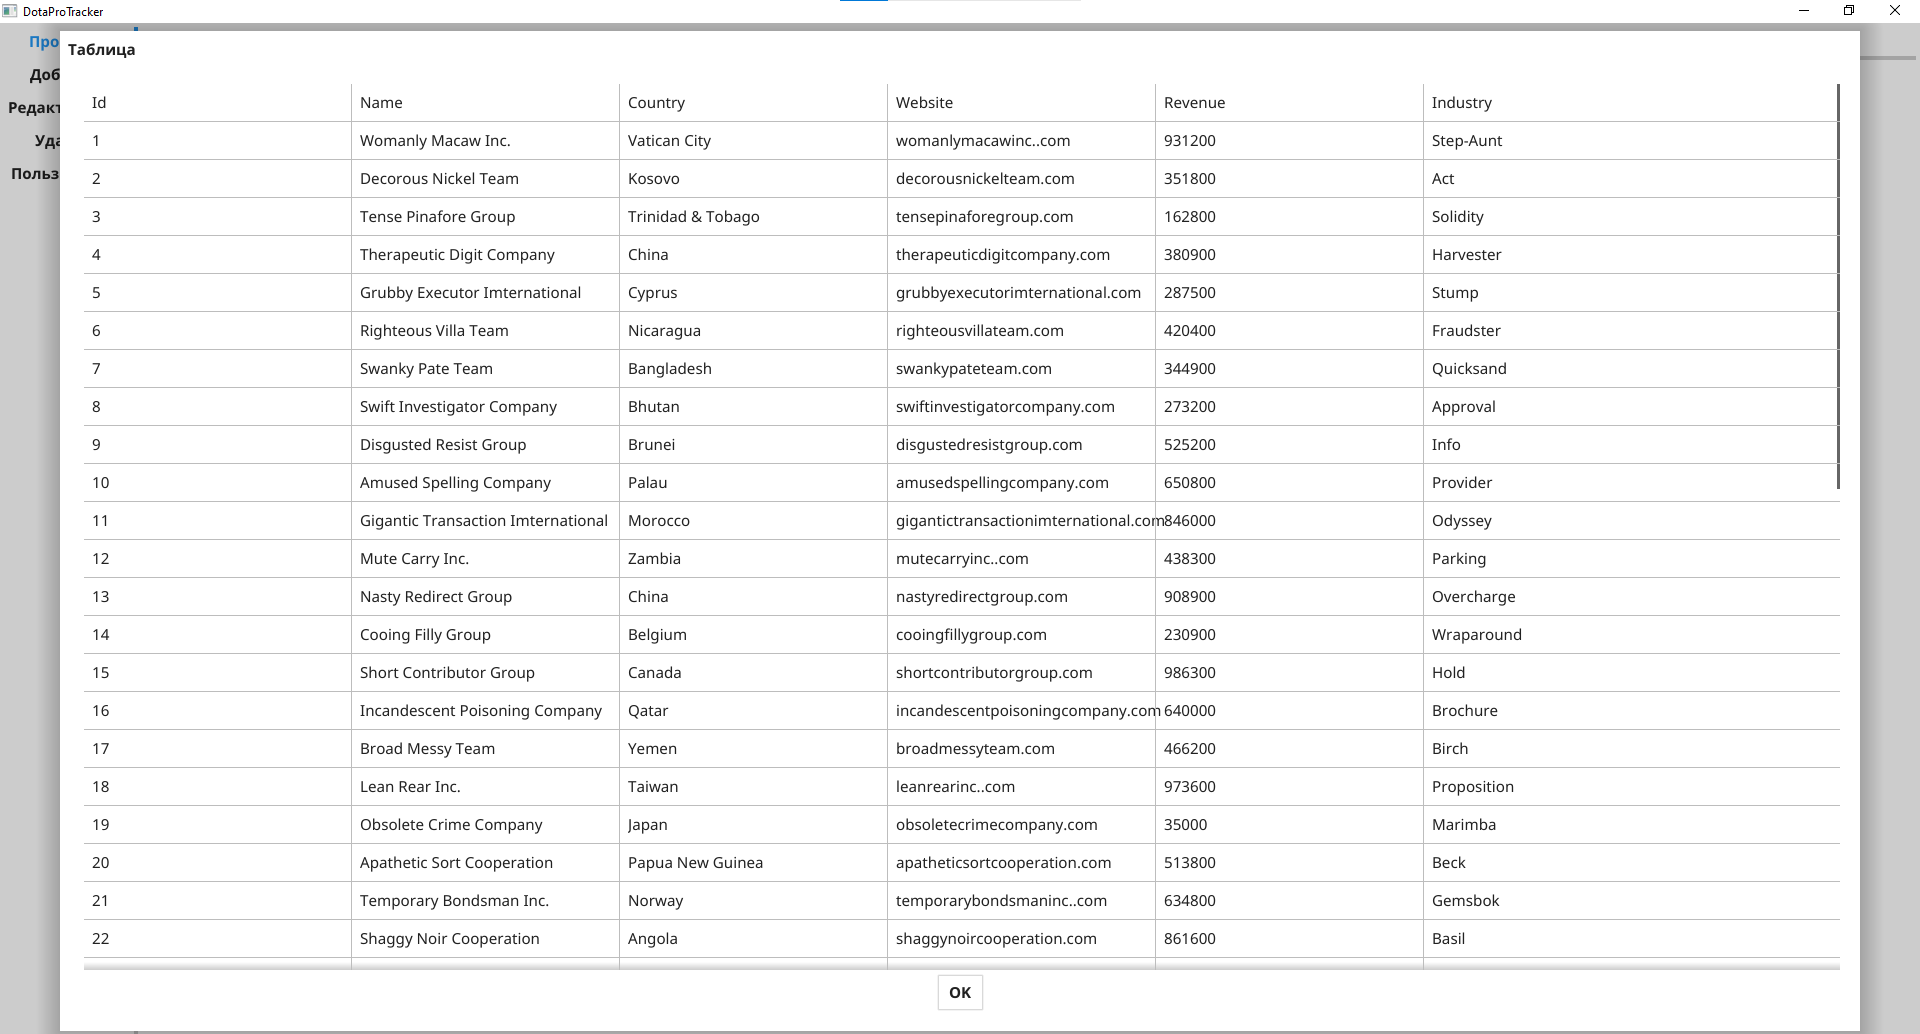
\includegraphics[scale = 0.3]{inc/img/companies.png}
	\caption{Просмотр записей о компаниях-спонсорах}
	\label{fig:companies}	
\end{figure}


\section*{Вывод}

В данном разделе были описаны выбранные технологии разработки, методология построения ПО, а также рассмотрено взаимодействие пользователя с приложением.''